\documentclass[12pt,a4paper]{article}

% ─── Packages ───────────────────────────────────────────────────────────────
\usepackage[a4paper, margin=2.5cm]{geometry}
\usepackage{amsmath, amssymb}
\usepackage{graphicx}
\usepackage{xcolor}
\usepackage{booktabs}
\usepackage{longtable}
\usepackage{array}
\usepackage{listings}
\usepackage{fancyhdr}
\usepackage{titlesec}
\usepackage{hyperref}
\usepackage{enumitem}
\usepackage{tikz}
\usetikzlibrary{shapes.geometric, arrows.meta, positioning, fit, backgrounds}
\usepackage{caption}
\usepackage{subcaption}
\usepackage{float}
\usepackage{tcolorbox}
\usepackage{multirow}
\usepackage{tabularx}
\usepackage{mdframed}

% ─── Colours ────────────────────────────────────────────────────────────────
\definecolor{primaryblue}{RGB}{10,80,160}
\definecolor{accentorange}{RGB}{220,100,20}
\definecolor{lightgray}{RGB}{245,245,245}
\definecolor{darkgray}{RGB}{60,60,60}
\definecolor{codebg}{RGB}{250,250,255}
\definecolor{codeframe}{RGB}{180,180,210}
\definecolor{passgreen}{RGB}{0,150,60}
\definecolor{warnred}{RGB}{200,30,30}

% ─── Hyperref ───────────────────────────────────────────────────────────────
\hypersetup{
    colorlinks=true,
    linkcolor=primaryblue,
    urlcolor=accentorange,
    citecolor=primaryblue,
    pdftitle={CipherStream-128X Design Report},
    pdfauthor={I-CHIP 26 PS-2}
}

% ─── Section Formatting ─────────────────────────────────────────────────────
\titleformat{\section}
  {\large\bfseries\color{primaryblue}}
  {\thesection}{1em}{}[\color{primaryblue}\titlerule]

\titleformat{\subsection}
  {\normalsize\bfseries\color{darkgray}}
  {\thesubsection}{1em}{}

\titleformat{\subsubsection}
  {\normalsize\bfseries\color{accentorange}}
  {\thesubsubsection}{1em}{}

% ─── Header / Footer ────────────────────────────────────────────────────────
\pagestyle{fancy}
\fancyhf{}
\renewcommand{\headrulewidth}{0.4pt}
\renewcommand{\footrulewidth}{0.4pt}
\fancyhead[L]{\small\color{darkgray} CipherStream-128X}
\fancyhead[R]{\small\color{darkgray} AES-128 Hardware Accelerator}
\fancyfoot[C]{\small\color{darkgray}\thepage}
\fancyfoot[R]{\small\color{darkgray} I-CHIP '26 --- PS-2}

% ─── Listings ───────────────────────────────────────────────────────────────
\lstdefinelanguage{verilog}{
  keywords={module, endmodule, input, output, wire, reg, always, assign,
            begin, end, if, else, case, endcase, posedge, negedge, parameter,
            function, endfunction, integer},
  keywordstyle=\color{primaryblue}\bfseries,
  commentstyle=\color{passgreen}\itshape,
  stringstyle=\color{accentorange},
  basicstyle=\ttfamily\footnotesize,
  breaklines=true,
  showstringspaces=false,
  numbers=left,
  numberstyle=\tiny\color{gray},
  frame=single,
  rulecolor=\color{codeframe},
  backgroundcolor=\color{codebg},
  xleftmargin=2em,
  framexleftmargin=1.5em,
  tabsize=4
}
\lstset{language=verilog}

% ─── Custom boxes ────────────────────────────────────────────────────────────
\newtcolorbox{infobox}[1][]{
  colback=lightgray, colframe=primaryblue,
  fonttitle=\bfseries\color{white},
  coltitle=white, title=#1,
  boxrule=0.8pt, arc=3pt
}

\newtcolorbox{warningbox}[1][]{
  colback=yellow!8, colframe=accentorange,
  fonttitle=\bfseries\color{white},
  coltitle=white, title=#1,
  boxrule=0.8pt, arc=3pt
}

% ─── TikZ arrow style ───────────────────────────────────────────────────────
\tikzset{
  block/.style={rectangle, draw=primaryblue, fill=blue!8,
                minimum width=2.2cm, minimum height=0.75cm,
                text centered, rounded corners=2pt, font=\small},
  pipe/.style={rectangle, draw=accentorange!80, fill=orange!10,
               minimum width=0.45cm, minimum height=0.75cm,
               text centered, font=\tiny},
  arr/.style={-Latex, thick, color=darkgray},
  dasharr/.style={-Latex, dashed, color=gray}
}

% ════════════════════════════════════════════════════════════════════════════
\begin{document}
% ════════════════════════════════════════════════════════════════════════════

% ─── Title Page ─────────────────────────────────────────────────────────────
\begin{titlepage}
\begin{center}
  \vspace*{1.5cm}
  {\Huge\bfseries\color{primaryblue} CipherStream-128X}\\[0.5em]
  {\Large\color{accentorange} AXI4-Enabled High-Throughput AES-128\\Hardware Accelerator}\\[2em]
  \hrule height 1pt
  \vspace{1em}
  {\large\bfseries Design Document \& Implementation Report}\\[0.5em]
  {\normalsize I-CHIP '26 --- Problem Statement 2\\
  Electronics Engineering Society, UDYAM '26}\\[2em]
  \hrule height 0.4pt
  \vspace{2em}

  \begin{tcolorbox}[colback=lightgray, colframe=primaryblue,
                   width=0.85\textwidth, arc=4pt]
    \centering
    \textbf{Design Summary}\\[0.5em]
    \begin{tabular}{ll}
      Architecture & Fully Pipelined AES-128 (ECB mode)\\
      Pipeline Depth & 11 stages (1 initial ARK + 9 rounds + 1 final round)\\
      Throughput & 1 block/clock cycle (steady state)\\
      Latency & 11 clock cycles\\
      Key Schedule & Precomputed, fully combinational\\
      S-box & LUT-based (256-entry \texttt{case} statement)\\
      AXI Interface & AXI4-Lite slave (config/key) + AXI-Stream\\
      HDL & Verilog (Vivado 2024.x)\\
    \end{tabular}
  \end{tcolorbox}

  \vfill
  {\small April 2026}
\end{center}
\end{titlepage}

% ─── Table of Contents ───────────────────────────────────────────────────────
\tableofcontents
\newpage

% ════════════════════════════════════════════════════════════════════════════
\section{Introduction}
% ════════════════════════════════════════════════════════════════════════════

This report documents the complete design and implementation of
\textbf{CipherStream-128X}, a hardware-based AES-128 cryptographic accelerator
built in Verilog and integrated via an AXI4-compliant IP interface.

The motivation arises from the inadequacy of software-based encryption in
high-throughput, latency-sensitive environments such as real-time sensor feeds,
telemetry streams, and control channels. Software encryption suffers from:
\begin{itemize}[nosep]
  \item High per-block latency and limited throughput.
  \item Susceptibility to timing-based side-channel attacks.
  \item Inability to sustain continuous, high-speed data streams.
\end{itemize}

The implemented accelerator addresses these limitations by:
\begin{enumerate}[nosep]
  \item Fully unrolling all 10 AES rounds into a hardware pipeline.
  \item Pre-computing the entire key schedule in combinational logic.
  \item Exposing the encryption core through AXI4-Lite (control/key) and
        AXI-Stream (data) interfaces for SoC integration.
\end{enumerate}

% ════════════════════════════════════════════════════════════════════════════
\section{AES-128 Algorithm Background}
% ════════════════════════════════════════════════════════════════════════════

AES-128 (FIPS-197) operates on a 128-bit state block with a 128-bit key over
10 rounds. Each round applies a sequence of invertible transformations to
achieve confusion and diffusion.

\subsection{Round Structure}

\begin{center}
\begin{tabular}{@{}cll@{}}
\toprule
\textbf{Round} & \textbf{Operations} & \textbf{Notes}\\
\midrule
0   & AddRoundKey                                       & Initial whitening\\
1--9 & SubBytes $\to$ ShiftRows $\to$ MixColumns $\to$ AddRoundKey & Full rounds\\
10  & SubBytes $\to$ ShiftRows $\to$ AddRoundKey        & Final round (no MixColumns)\\
\bottomrule
\end{tabular}
\end{center}

\vspace{0.5em}

\begin{description}[nosep, leftmargin=2cm, style=nextline]
  \item[\textbf{SubBytes}] Non-linear byte substitution using the AES S-box
        (affine transformation over GF($2^8$)).
  \item[\textbf{ShiftRows}] Cyclic left-rotation of each row of the 4×4 state
        matrix by 0, 1, 2, 3 positions respectively.
  \item[\textbf{MixColumns}] Matrix multiplication over GF($2^8$) with the
        fixed MDS matrix $[2,3,1,1]$ (and cyclic rotations) applied per column.
  \item[\textbf{AddRoundKey}] Bitwise XOR of the state with the current round key.
\end{description}

% ════════════════════════════════════════════════════════════════════════════
\section{Top-Level Architecture}
% ════════════════════════════════════════════════════════════════════════════

\subsection{Design Hierarchy}

The design is organised into three layers:

\begin{center}
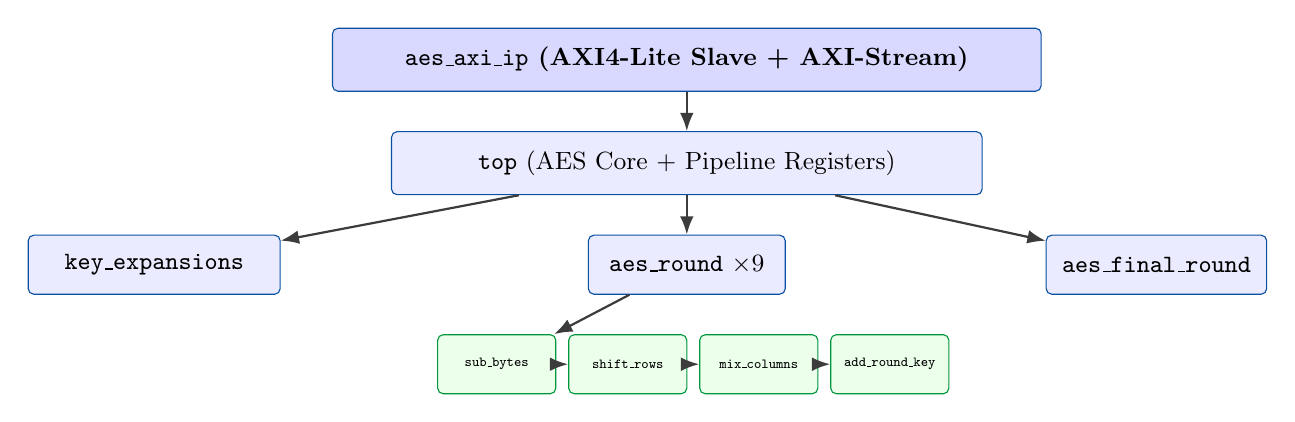
\begin{tikzpicture}[node distance=0.4cm and 0.6cm]

  % AXI wrapper
  \node[block, minimum width=9cm, minimum height=0.8cm,
        fill=blue!15, draw=primaryblue, font=\bfseries\small]
    (axi) {\texttt{aes\_axi\_ip}  \small(AXI4-Lite Slave + AXI-Stream)};

  % Top
  \node[block, minimum width=7.5cm, minimum height=0.8cm,
        fill=blue!8, below=0.5cm of axi]
    (top) {\texttt{top}  \small(AES Core + Pipeline Registers)};

  % Key expansions
  \node[block, minimum width=3.2cm, below left=0.5cm and 1.4cm of top]
    (ke) {\texttt{key\_expansions}};

  % aes_round
  \node[block, minimum width=2.5cm, below=0.5cm of top]
    (ar) {\texttt{aes\_round} $\times 9$};

  % final round
  \node[block, minimum width=2.8cm, below right=0.5cm and 0.8cm of top]
    (fr) {\texttt{aes\_final\_round}};

  % sub-modules of aes_round
  \node[block, fill=green!8, draw=passgreen, minimum width=1.5cm,
        below left=0.5cm and 0.4cm of ar, font=\tiny]
    (sb) {\texttt{sub\_bytes}};
  \node[block, fill=green!8, draw=passgreen, minimum width=1.5cm,
        right=0.15cm of sb, font=\tiny]
    (sr) {\texttt{shift\_rows}};
  \node[block, fill=green!8, draw=passgreen, minimum width=1.5cm,
        right=0.15cm of sr, font=\tiny]
    (mc) {\texttt{mix\_columns}};
  \node[block, fill=green!8, draw=passgreen, minimum width=1.5cm,
        right=0.15cm of mc, font=\tiny]
    (ark) {\texttt{add\_round\_key}};

  % arrows
  \draw[arr] (axi) -- (top);
  \draw[arr] (top) -- (ke);
  \draw[arr] (top) -- (ar);
  \draw[arr] (top) -- (fr);
  \draw[arr] (ar)  -- (sb);
  \draw[arr] (sb)  -- (sr);
  \draw[arr] (sr)  -- (mc);
  \draw[arr] (mc)  -- (ark);

\end{tikzpicture}
\end{center}

\subsection{Module Inventory}

\begin{table}[H]
\centering
\begin{tabularx}{\textwidth}{@{}llX@{}}
\toprule
\textbf{Module} & \textbf{File} & \textbf{Role}\\
\midrule
\texttt{aes\_axi\_ip}       & \texttt{aes\_axi.v}            & AXI4-Lite config/key slave + AXI-Stream data path\\
\texttt{top}                & \texttt{top.v}                 & 11-stage pipeline, valid tracking, output register\\
\texttt{key\_expansions}    & \texttt{key\_expansions.v}     & Fully combinational key schedule (K0--K10)\\
\texttt{key\_expansion\_round} & \texttt{key\_expansion\_round.v} & One AES key expansion step with inline S-box\\
\texttt{aes\_round}         & \texttt{aes\_round.v}          & Full round: SubBytes$\to$ShiftRows$\to$MixColumns$\to$ARK\\
\texttt{aes\_final\_round}  & \texttt{aes\_final\_round.v}   & Final round: SubBytes$\to$ShiftRows$\to$ARK\\
\texttt{sub\_bytes}         & \texttt{sub\_bytes.v}          & 16 parallel byte substitutions (LUT S-box)\\
\texttt{shift\_rows}        & \texttt{ShiftRows.v}           & Combinational byte permutation\\
\texttt{mix\_columns}       & \texttt{mix\_columns.v}        & GF($2^8$) column mixing\\
\texttt{add\_round\_key}    & \texttt{add\_round\_key.v}     & 128-bit XOR\\
\bottomrule
\end{tabularx}
\end{table}

% ════════════════════════════════════════════════════════════════════════════
\section{Pipeline Architecture}
% ════════════════════════════════════════════════════════════════════════════

\subsection{Pipeline Structure}

The core is implemented in \texttt{top.v} as a \textbf{fully unrolled,
11-stage synchronous pipeline}. Each pipeline stage corresponds to one AES
transformation step, separated by a 128-bit flip-flop register.

\begin{figure}[H]
\centering
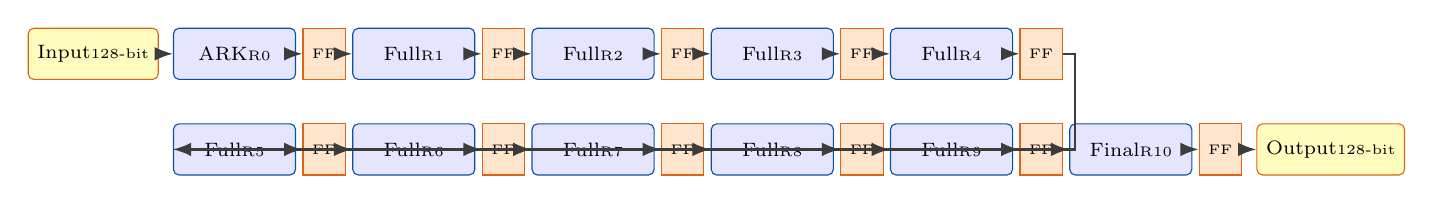
\begin{tikzpicture}[
  stg/.style={rectangle, draw=primaryblue, fill=blue!10,
              minimum width=1.55cm, minimum height=0.65cm,
              text centered, font=\scriptsize, rounded corners=2pt},
  ff/.style={rectangle, draw=accentorange, fill=orange!20,
             minimum width=0.35cm, minimum height=0.65cm,
             text centered, font=\tiny},
  inarr/.style={-Latex, thick, color=darkgray}
]
  % Nodes
  \node[stg, fill=yellow!25, draw=accentorange] (in) {Input\\[-1pt]\tiny 128-bit};
  \node[stg, right=0.18cm of in]  (s0)  {ARK\\[-1pt]\tiny R0};
  \node[ff,  right=0.08cm of s0]  (r0)  {FF};
  \node[stg, right=0.08cm of r0]  (s1)  {Full\\[-1pt]\tiny R1};
  \node[ff,  right=0.08cm of s1]  (r1)  {FF};
  \node[stg, right=0.08cm of r1]  (s2)  {Full\\[-1pt]\tiny R2};
  \node[ff,  right=0.08cm of s2]  (r2)  {FF};
  \node[stg, right=0.08cm of r2]  (s3)  {Full\\[-1pt]\tiny R3};
  \node[ff,  right=0.08cm of s3]  (r3)  {FF};
  \node[stg, right=0.08cm of r3]  (s4)  {Full\\[-1pt]\tiny R4};
  \node[ff,  right=0.08cm of s4]  (r4)  {FF};

  % Second row
  \node[stg, below=0.55cm of s0]  (s5)  {Full\\[-1pt]\tiny R5};
  \node[ff,  right=0.08cm of s5]  (r5)  {FF};
  \node[stg, right=0.08cm of r5]  (s6)  {Full\\[-1pt]\tiny R6};
  \node[ff,  right=0.08cm of s6]  (r6)  {FF};
  \node[stg, right=0.08cm of r6]  (s7)  {Full\\[-1pt]\tiny R7};
  \node[ff,  right=0.08cm of s7]  (r7)  {FF};
  \node[stg, right=0.08cm of r7]  (s8)  {Full\\[-1pt]\tiny R8};
  \node[ff,  right=0.08cm of s8]  (r8)  {FF};
  \node[stg, right=0.08cm of r8]  (s9)  {Full\\[-1pt]\tiny R9};
  \node[ff,  right=0.08cm of s9]  (r9)  {FF};
  \node[stg, right=0.08cm of r9]  (s10) {Final\\[-1pt]\tiny R10};
  \node[ff,  right=0.08cm of s10] (ro)  {FF};
  \node[stg, fill=yellow!25, draw=accentorange,
        right=0.18cm of ro] (out) {Output\\[-1pt]\tiny 128-bit};

  % Arrows row 1
  \draw[inarr] (in) -- (s0);
  \draw[inarr] (s0) -- (r0); \draw[inarr] (r0) -- (s1);
  \draw[inarr] (s1) -- (r1); \draw[inarr] (r1) -- (s2);
  \draw[inarr] (s2) -- (r2); \draw[inarr] (r2) -- (s3);
  \draw[inarr] (s3) -- (r3); \draw[inarr] (r3) -- (s4);
  \draw[inarr] (s4) -- (r4);

  % Bend down from r4 to s5
  \draw[inarr] (r4.east) -- ++(0.15,0) |- (s5.west);

  % Arrows row 2
  \draw[inarr] (s5) -- (r5); \draw[inarr] (r5) -- (s6);
  \draw[inarr] (s6) -- (r6); \draw[inarr] (r6) -- (s7);
  \draw[inarr] (s7) -- (r7); \draw[inarr] (r7) -- (s8);
  \draw[inarr] (s8) -- (r8); \draw[inarr] (r8) -- (s9);
  \draw[inarr] (s9) -- (r9); \draw[inarr] (r9) -- (s10);
  \draw[inarr] (s10) -- (ro); \draw[inarr] (ro) -- (out);

\end{tikzpicture}
\caption{11-Stage AES-128 Encryption Pipeline (FF = 128-bit flip-flop register)}
\end{figure}

\subsection{Pipeline Register Management}

In \texttt{top.v}, the pipeline registers \texttt{s0}--\texttt{s9} are
declared as 128-bit regs and updated on every rising clock edge:

\begin{itemize}[nosep]
  \item \textbf{\texttt{s0}} is loaded from the output of the initial
        AddRoundKey (\texttt{r0\_out}) only when \texttt{s\_axis\_tvalid}
        is asserted, preventing stale data from propagating.
  \item \textbf{\texttt{s1}--\texttt{s9}} are updated unconditionally from
        their predecessor round outputs on every clock.
  \item \textbf{\texttt{s10}} captures the final-round output
        (\texttt{r10\_out}) every cycle.
\end{itemize}

\subsection{Valid Signal Propagation}

A dedicated 11-bit shift register \texttt{valid\_pipe[10:0]} shadows the
data as it flows through the pipeline:

\begin{lstlisting}[caption={Valid pipeline shift register}]
valid_pipe <= {valid_pipe[9:0], s_axis_tvalid};
\end{lstlisting}

When \texttt{valid\_pipe[10]} is asserted, the corresponding ciphertext is
guaranteed to be present in \texttt{s10}, and the output register
\texttt{out\_data\_reg} is updated.

\subsection{Output Handshake}

The output stage implements a simple ready/valid register:

\begin{lstlisting}[caption={AXI-Stream output register with backpressure}]
if (m_axis_tready || !out_valid_reg) begin
    out_data_reg  <= s10;
    out_valid_reg <= valid_pipe[10];
end
\end{lstlisting}

This ensures the output ciphertext is held stable until the downstream
consumer asserts \texttt{m\_axis\_tready}, providing basic backpressure
support on the output side.

\subsection{Input Path}

The input \texttt{s\_axis\_tready} is permanently tied high:
\begin{lstlisting}
assign s_axis_tready = 1'b1;
\end{lstlisting}

This means the accelerator can accept a new 128-bit block on every single
clock cycle, achieving \textbf{1 block/cycle} throughput in steady state.
The pipeline will contain up to 11 blocks in flight simultaneously.

% ════════════════════════════════════════════════════════════════════════════
\section{Module-Level Design Details}
% ════════════════════════════════════════════════════════════════════════════

\subsection{SubBytes (\texttt{sub\_bytes.v})}

\subsubsection{Implementation Strategy: LUT-Based S-box}

The SubBytes transformation is implemented as a \textbf{256-entry lookup
table} using a Verilog \texttt{case} statement inside a function
\texttt{sbox(in)}. This function is then applied to all 16 bytes of the
128-bit state in parallel via 16 concurrent \texttt{assign} statements:

\begin{lstlisting}[caption={Parallel byte-wise S-box application}]
assign data_out[7:0]     = sbox(data_in[7:0]);
assign data_out[15:8]    = sbox(data_in[15:8]);
// ... (16 total, bytes [7:0] through [127:120])
\end{lstlisting}

\subsubsection{Tradeoff Analysis}

\begin{table}[H]
\centering
\begin{tabular}{@{}lll@{}}
\toprule
\textbf{Approach} & \textbf{Pros} & \textbf{Cons}\\
\midrule
LUT (case, chosen) & Zero propagation delay; synthesiser-friendly & Higher LUT count\\
Composite field GF & Minimal area & More complex; harder to verify\\
BRAM-based         & Saves logic & Adds read latency; BRAM pressure\\
\bottomrule
\end{tabular}
\end{table}

The LUT approach was chosen for its simplicity, correctness guarantees, and
the fact that modern FPGAs natively implement \texttt{case}-based logic as
efficient 6-input LUTs.

\subsection{ShiftRows (\texttt{ShiftRows.v})}

ShiftRows is implemented as a \textbf{pure combinational byte permutation}.
The 128-bit state is treated as a 4$\times$4 byte matrix (row-major). Each
row is cyclically left-shifted by its row index (0, 1, 2, 3 bytes):

\begin{lstlisting}[caption={ShiftRows byte permutation}]
assign data_out = {
    b0,  b5,  b10, b15,   // Row 0: no shift
    b4,  b9,  b14, b3,    // Row 1: left-shift 1
    b8,  b13, b2,  b7,    // Row 2: left-shift 2
    b12, b1,  b6,  b11    // Row 3: left-shift 3
};
\end{lstlisting}

This is a \textbf{zero-cost} operation in hardware---it resolves entirely
as a wiring permutation with no gates required.

\subsection{MixColumns (\texttt{mix\_columns.v})}

\subsubsection{GF($2^8$) Arithmetic}

MixColumns multiplies each 4-byte column by the fixed MDS matrix over
GF($2^8$) with the irreducible polynomial $x^8 + x^4 + x^3 + x + 1$
(0x11B). The multiplication by 2 (\texttt{mul2}) and by 3 (\texttt{mul3})
are implemented as helper functions:

\begin{lstlisting}[caption={GF(2\^{}8) multiplication helper functions}]
function [7:0] mul2;
    input [7:0] x;
    begin
        mul2 = (x[7]) ? ((x << 1) ^ 8'h1b) : (x << 1);
    end
endfunction

function [7:0] mul3;
    input [7:0] x;
    begin
        mul3 = mul2(x) ^ x;   // mul3 = mul2 XOR identity
    end
endfunction
\end{lstlisting}

\subsubsection{Column Computation}

Each output byte of a column is computed according to the MDS matrix:

\[
\begin{pmatrix} c_0 \\ c_1 \\ c_2 \\ c_3 \end{pmatrix}
=
\begin{pmatrix} 2 & 3 & 1 & 1 \\ 1 & 2 & 3 & 1 \\
                1 & 1 & 2 & 3 \\ 3 & 1 & 1 & 2 \end{pmatrix}
\begin{pmatrix} b_0 \\ b_1 \\ b_2 \\ b_3 \end{pmatrix}
\quad \text{over GF}(2^8)
\]

All four columns are computed in parallel, making this a fully
combinational, zero-latency operation.

\subsection{AddRoundKey (\texttt{add\_round\_key.v})}

The simplest of all transformations---a single 128-bit XOR:

\begin{lstlisting}[caption={AddRoundKey implementation}]
assign data_out = data_in ^ round_key;
\end{lstlisting}

\subsection{AES Round (\texttt{aes\_round.v})}

The full AES round (rounds 1--9) instantiates the four sub-modules in a
\textbf{combinational chain} with no intermediate registers:

\begin{center}
\texttt{data\_in}
$\xrightarrow{\text{sub\_bytes}}$
$\xrightarrow{\text{shift\_rows}}$
$\xrightarrow{\text{mix\_columns}}$
$\xrightarrow{\text{add\_round\_key}}$
\texttt{data\_out}
\end{center}

The round is entirely combinational; the pipeline register sits in
\texttt{top.v} at the stage boundary.

\subsection{AES Final Round (\texttt{aes\_final\_round.v})}

Round 10 omits MixColumns as per FIPS-197:

\begin{center}
\texttt{data\_in}
$\xrightarrow{\text{sub\_bytes}}$
$\xrightarrow{\text{shift\_rows}}$
$\xrightarrow{\text{add\_round\_key}}$
\texttt{data\_out}
\end{center}

% ════════════════════════════════════════════════════════════════════════════
\section{Key Schedule}
% ════════════════════════════════════════════════════════════════════════════

\subsection{Strategy: Precomputed Combinational Key Schedule}

The key schedule adopts the \textbf{precomputed} approach: all 11 round keys
(K0--K10) are derived from the initial 128-bit key in a single chain of
combinational logic with no clock dependence. The 128-bit key is presented
to \texttt{key\_expansions} and all 11 round keys are available within the
combinational propagation delay.

\subsection{\texttt{key\_expansion\_round} Module}

Each round of key expansion performs:

\begin{enumerate}[nosep]
  \item \textbf{RotWord:} Left-rotate the last word (W3) by one byte.
  \item \textbf{SubWord:} Apply the AES S-box to each byte of the rotated word.
        (The S-box is inlined as a function identical to \texttt{sub\_bytes}.)
  \item \textbf{RCON XOR:} XOR with the round constant for the current round.
  \item \textbf{Word XOR chain:} $W4 = W0 \oplus \text{temp}$,\ \ $W5 = W1 \oplus W4$,\ \ $W6 = W2 \oplus W5$,\ \ $W7 = W3 \oplus W6$.
\end{enumerate}

The 10 round constants are pre-encoded as a \texttt{case} statement:

\begin{lstlisting}[caption={RCON lookup table (rounds 1--10)}]
4'd1:  rcon = 32'h01000000;  4'd2:  rcon = 32'h02000000;
4'd3:  rcon = 32'h04000000;  4'd4:  rcon = 32'h08000000;
4'd5:  rcon = 32'h10000000;  4'd6:  rcon = 32'h20000000;
4'd7:  rcon = 32'h40000000;  4'd8:  rcon = 32'h80000000;
4'd9:  rcon = 32'h1b000000;  4'd10: rcon = 32'h36000000;
\end{lstlisting}

\subsection{\texttt{key\_expansions} Module}

Ten instances of \texttt{key\_expansion\_round} are chained combinationally:

\begin{lstlisting}[caption={Unrolled key expansion chain}]
assign K0 = key_initial;
key_expansion_round r1 (.input_key(K0), .round(4'd1),  .output_key(K1));
key_expansion_round r2 (.input_key(K1), .round(4'd2),  .output_key(K2));
// ... r3 through r10 similarly
assign round_keys = {K0,K1,K2,K3,K4,K5,K6,K7,K8,K9,K10};  // 1408-bit bus
\end{lstlisting}

The output is a single 1408-bit concatenated wire, which \texttt{top.v}
slices into 11 individual 128-bit round key wires:

\begin{lstlisting}[caption={Round key slicing in top.v}]
wire [127:0] K0  = round_keys[1407:1280];
wire [127:0] K1  = round_keys[1279:1152];
// ...
wire [127:0] K10 = round_keys[127:0];
\end{lstlisting}

\subsection{Key Schedule Tradeoffs}

\begin{table}[H]
\centering
\begin{tabular}{@{}llll@{}}
\toprule
\textbf{Strategy} & \textbf{Latency} & \textbf{Area} & \textbf{Dynamic Key Support}\\
\midrule
Precomputed (chosen) & Zero (combinational) & Higher LUT usage & Yes (new key → new output next cycle)\\
On-the-fly           & 10 cycles            & Lower           & Requires pipeline stall\\
BRAM-stored          & 1 cycle read         & Minimal logic   & Needs write port + synchronisation\\
\bottomrule
\end{tabular}
\end{table}

The precomputed strategy is optimal for a fully pipelined design: since the
key schedule is combinational, any change to the \texttt{key} input is
reflected in all round keys within one propagation delay. Because new
plaintext blocks sample the round keys only at clock edges, this is safe as
long as the key is held stable for the duration of a streaming burst.

% ════════════════════════════════════════════════════════════════════════════
\section{AXI Interface Design}
% ════════════════════════════════════════════════════════════════════════════

\subsection{Overview}

The \texttt{aes\_axi\_ip} wrapper exposes two interfaces:

\begin{enumerate}[nosep]
  \item \textbf{AXI4-Lite Slave} --- for configuration (start/stop) and key
        loading.
  \item \textbf{AXI-Stream} --- for high-throughput plaintext/ciphertext data
        transfer (passed through to \texttt{top}).
\end{enumerate}

\subsection{AXI4-Lite Register Map}

\begin{table}[H]
\centering
\begin{tabular}{@{}llll@{}}
\toprule
\textbf{Offset} & \textbf{Name} & \textbf{Access} & \textbf{Description}\\
\midrule
\texttt{0x00} & \texttt{CTRL}     & R/W & Bit[0] = \texttt{start} (write 1 to start, 0 to stop)\\
\texttt{0x04} & \texttt{STATUS}   & R   & Bit[0] = \texttt{done} (asserted when first output valid)\\
\texttt{0x10} & \texttt{KEY[127:96]} & W & Most-significant 32 bits of key\\
\texttt{0x14} & \texttt{KEY[95:64]}  & W & Second word of key\\
\texttt{0x18} & \texttt{KEY[63:32]}  & W & Third word of key\\
\texttt{0x1C} & \texttt{KEY[31:0]}   & W & Least-significant 32 bits of key\\
\bottomrule
\end{tabular}
\caption{AXI4-Lite register map of \texttt{aes\_axi\_ip}}
\end{table}

The 128-bit AES key is written through four consecutive 32-bit word writes.
This mapping allows any AXI-Lite master (processor, DMA controller) to
configure the accelerator using standard 32-bit memory-mapped writes.

\subsection{Write Path}

Write address and write data channels are accepted simultaneously
(\texttt{s\_axi\_awvalid \&\& s\_axi\_wvalid}). All three ready signals
(\texttt{awready}, \texttt{wready}, \texttt{arready}) are permanently
asserted:

\begin{lstlisting}[caption={Always-ready AXI4-Lite handshake}]
assign s_axi_awready = 1'b1;
assign s_axi_wready  = 1'b1;
assign s_axi_arready = 1'b1;
\end{lstlisting}

A write response (\texttt{bvalid}) is generated on the cycle following a
successful write and held until \texttt{bready} is seen.

\subsection{Read Path}

Read data is registered on the cycle following an \texttt{arvalid} assertion.
The register file supports read-back of all configuration registers,
allowing the host to verify key loading.

\subsection{Status Register}

The \texttt{done} bit provides a lightweight completion indicator:
\begin{itemize}[nosep]
  \item Clears to 0 when \texttt{start} is asserted.
  \item Sets to 1 upon the first valid output from the AES pipeline
        (\texttt{core\_valid\_out}).
\end{itemize}

\begin{warningbox}[Implementation Note]
The current implementation does not include \texttt{Busy} or \texttt{Error}
status bits as separate register fields. The \texttt{done} bit serves as the
primary completion indicator. Since \texttt{s\_axis\_tready} is permanently
high, the pipeline never signals busy to upstream producers.
\end{warningbox}

\subsection{AXI-Stream Interface}

Data flows through the AXI-Stream interface:

\begin{center}
\begin{tabular}{@{}lll@{}}
\toprule
\textbf{Signal} & \textbf{Direction} & \textbf{Description}\\
\midrule
\texttt{s\_axis\_tdata[127:0]}  & Input  & 128-bit plaintext block\\
\texttt{s\_axis\_tvalid}         & Input  & Plaintext valid\\
\texttt{s\_axis\_tready}         & Output & Always 1 (never stalls)\\
\texttt{m\_axis\_tdata[127:0]}  & Output & 128-bit ciphertext block\\
\texttt{m\_axis\_tvalid}         & Output & Ciphertext valid (11 cycles after input)\\
\texttt{m\_axis\_tready}         & Input  & Downstream consumer ready\\
\bottomrule
\end{tabular}
\end{center}

% ════════════════════════════════════════════════════════════════════════════
\section{Verification \& Testbench}
% ════════════════════════════════════════════════════════════════════════════

\subsection{Testbench Suite}

Six testbenches cover individual modules and the full system:

\begin{table}[H]
\centering
\begin{tabularx}{\textwidth}{@{}llX@{}}
\toprule
\textbf{Testbench} & \textbf{DUT} & \textbf{Coverage}\\
\midrule
\texttt{tb\_sub\_bytes.v}           & \texttt{sub\_bytes}         & Single-byte S-box: input \texttt{0x53} $\to$ expected \texttt{0xED}\\
\texttt{tb\_mix\_columns.v}         & \texttt{mix\_columns}       & Full 128-bit MixColumns output check\\
\texttt{tb\_aes\_round.v}           & \texttt{aes\_round}         & Single full round with FIPS-197 test vector\\
\texttt{tb\_key\_expansion\_round.v}& \texttt{key\_expansion\_round} & Key expansion round 1: \texttt{0x2b7e...} $\to$ \texttt{0xa0fa...}\\
\texttt{tb\_top.v}                  & \texttt{top}                & End-to-end AES-128 FIPS-197 test vector verification\\
\texttt{tb\_aes\_pipeline.v}        & \texttt{top}                & Pipelined streaming: 4 consecutive identical blocks\\
\bottomrule
\end{tabularx}
\end{table}

\subsection{FIPS-197 Standard Test Vector}

The primary correctness check uses the standard FIPS-197 Appendix B test vector:

\begin{infobox}[FIPS-197 Test Vector]
\begin{tabular}{ll}
\textbf{Plaintext:} & \texttt{00112233 44556677 8899aabb ccddeeff}\\
\textbf{Key:}       & \texttt{00010203 04050607 08090a0b 0c0d0e0f}\\
\textbf{Expected:}  & \texttt{69c4e0d8 6a7b0430 d8cdb780 70b4c55a}\\
\end{tabular}
\end{infobox}

This is verified in both \texttt{tb\_top.v} (combinational path check) and
\texttt{tb\_aes\_pipeline.v} (clocked pipeline check):

\begin{lstlisting}[caption={Pass/fail check in tb\_top.v}]
if (output_data == 128'h69c4e0d86a7b0430d8cdb78070b4c55a)
    $display("AES TEST PASSED");
else begin
    $display("AES TEST FAILED");
    $display("Expected = 69c4e0d86a7b0430d8cdb78070b4c55a");
end
\end{lstlisting}

\subsection{Key Expansion Verification}

\texttt{tb\_key\_expansion\_round.v} verifies round 1 of the key schedule
with the standard FIPS-197 key schedule test:

\begin{infobox}[Key Expansion Test Vector]
\begin{tabular}{ll}
\textbf{Input Key:}   & \texttt{2b7e1516 28aed2a6 abf71588 09cf4f3c}\\
\textbf{Expected K1:} & \texttt{a0fafe17 88542cb1 23a33939 2a6c7605}\\
\end{tabular}
\end{infobox}

\subsection{Pipeline Streaming Test}

\texttt{tb\_aes\_pipeline.v} feeds 4 identical plaintext blocks
back-to-back into the pipeline and checks that all 4 corresponding
ciphertext outputs match the expected value, validating sustained
throughput and the validity tracking logic.

% ════════════════════════════════════════════════════════════════════════════
\section{Performance Analysis}
% ════════════════════════════════════════════════════════════════════════════

\subsection{Latency}

The end-to-end pipeline latency is \textbf{11 clock cycles}:

\begin{center}
\begin{tabular}{@{}clc@{}}
\toprule
\textbf{Stage} & \textbf{Operation} & \textbf{Cycles}\\
\midrule
0   & AddRoundKey (initial whitening) + register & 1\\
1--9 & 9$\times$ full AES round + register each & 9\\
10  & Final round + output register              & 1\\
\midrule
\textbf{Total} & & \textbf{11}\\
\bottomrule
\end{tabular}
\end{center}

With a target clock of $f$ MHz, the latency in nanoseconds is
$T_\text{lat} = 11 / f \times 10^3$\,ns. For example, at 200\,MHz:
$T_\text{lat} = 55$\,ns.

\subsection{Throughput}

Since the pipeline accepts one new 128-bit block per clock cycle in steady
state:

\[
\text{Throughput} = f \times 128\ \text{bits/cycle} = 128f\ \text{Mbps}
\]

At 200\,MHz: $\text{Throughput} = 25.6\ \text{Gbps}$.

\begin{table}[H]
\centering
\begin{tabular}{@{}lll@{}}
\toprule
\textbf{Clock Frequency} & \textbf{Throughput} & \textbf{Latency}\\
\midrule
100 MHz & 12.8 Gbps & 110 ns (11 cycles)\\
200 MHz & 25.6 Gbps & 55 ns\\
300 MHz & 38.4 Gbps & 36.7 ns\\
\bottomrule
\end{tabular}
\caption{Estimated performance at various clock frequencies}
\end{table}

The achievable $F_{\max}$ is bounded by the critical path through a single
AES round: SubBytes (S-box LUT) $\to$ ShiftRows (wires) $\to$ MixColumns
(GF arithmetic) $\to$ AddRoundKey (XOR). On a Xilinx 7-series FPGA, this
is typically in the range of 150--250\,MHz depending on placement.

\subsection{Resource Utilization Estimates}

\begin{table}[H]
\centering
\begin{tabular}{@{}lll@{}}
\toprule
\textbf{Resource} & \textbf{Estimated Usage} & \textbf{Notes}\\
\midrule
LUTs       & $\sim$3,500--5,000 & Dominated by 16 S-box LUTs $\times$ 11 rounds\\
Flip-Flops & $\sim$1,408        & 11 pipeline stages $\times$ 128 bits each\\
BRAM       & 0                  & All storage is in registers (no BRAM used)\\
DSPs       & 0                  & GF arithmetic uses LUT logic only\\
\bottomrule
\end{tabular}
\caption{Estimated FPGA resource utilization (Xilinx 7-series target)}
\end{table}

% ════════════════════════════════════════════════════════════════════════════
\section{Design Tradeoff Analysis}
% ════════════════════════════════════════════════════════════════════════════

\subsection{Fully Pipelined vs.\ Iterative}

The chosen fully-unrolled pipeline achieves maximum throughput (1 block/cycle)
at the cost of area---11 instantiations of the round logic are required.
An iterative architecture using a single round with a feedback register would
reduce area by $\sim$10$\times$ but would also reduce throughput to
1 block/10 cycles and introduce control complexity.

\subsection{S-box Implementation}

LUT-based S-boxes (chosen) synthesise efficiently on FPGAs where each
6-input LUT can store 64 bits of truth table. Composite-field implementations
reduce area on ASICs but add logic depth, which may reduce $F_{\max}$.

\subsection{Key Schedule Architecture}

The fully combinational key schedule eliminates any need to pre-buffer or
serialise round keys. The tradeoff is a longer critical path from the key
input to the round key outputs, but since this path is not in the data
pipeline, it does not limit throughput directly.

\subsection{Always-Ready Input (\texttt{s\_axis\_tready = 1})}

Tying the input ready permanently high simplifies upstream producer logic
and maximises throughput. It assumes the upstream producer respects the
valid signal and does not send invalid data on cycles when
\texttt{tvalid} is low. The valid-pipe mechanism in \texttt{top.v} correctly
handles gaps in input valid.

% ════════════════════════════════════════════════════════════════════════════
\section{Known Limitations \& Future Work}
% ════════════════════════════════════════════════════════════════════════════

\begin{enumerate}
  \item \textbf{Decryption not implemented.} The current design supports
        encryption only (ECB mode). Decryption requires inverse S-box,
        inverse ShiftRows, and inverse MixColumns.

  \item \textbf{CBC/CTR modes not implemented.} Only ECB mode is present.
        CTR mode (preferred for streaming) would require adding a counter and
        XOR stage before the AES core; CBC requires a feedback register.

  \item \textbf{Key update safety.} The combinational key schedule means that
        mid-stream key changes affect all in-flight pipeline stages
        simultaneously. A production system should hold the key stable for
        at least 11 cycles after the last block of a burst, or register the
        key separately into each pipeline stage.

  \item \textbf{No AXI-Stream slave memory.} The PS requires a companion
        AXI4-Lite compliant slave memory. This block (\texttt{design\_1} in
        the Vivado hierarchy) is present as a block design but not as a
        custom RTL module in the submitted sources.

  \item \textbf{Status register completeness.} The \texttt{Busy} and
        \texttt{Error} status bits specified in the PS interface are not
        explicitly implemented as addressable register bits.

  \item \textbf{Synthesis not run.} Reported resource figures are estimates;
        actual synthesis results on the target device are pending.
\end{enumerate}

% ════════════════════════════════════════════════════════════════════════════
\section{Conclusion}
% ════════════════════════════════════════════════════════════════════════════

CipherStream-128X successfully implements a \textbf{fully pipelined,
stall-free AES-128 encryption engine} in Verilog, integrated within an
AXI4-Lite compliant IP wrapper. The design achieves:

\begin{itemize}[nosep]
  \item 1 block/cycle throughput in steady state.
  \item 11-cycle deterministic latency.
  \item Zero BRAM usage --- all state held in pipeline flip-flops.
  \item LUT-based S-box for predictable, timing-attack-resistant operation.
  \item Fully combinational precomputed key schedule.
  \item Correct output verified against the FIPS-197 standard test vector.
\end{itemize}

The architecture demonstrates a clean separation of concerns: the
cryptographic datapath (\texttt{top.v} and its sub-modules) is independent
of the bus interface (\texttt{aes\_axi\_ip}), making the core portable to
any AXI-based SoC.

% ════════════════════════════════════════════════════════════════════════════
\appendix
\section{File Manifest}
% ════════════════════════════════════════════════════════════════════════════

\begin{table}[H]
\centering
\begin{tabular}{@{}lll@{}}
\toprule
\textbf{File} & \textbf{Type} & \textbf{Role}\\
\midrule
\texttt{aes\_axi.v}             & Design & AXI4-Lite + AXI-Stream wrapper\\
\texttt{top.v}                  & Design & Pipeline top level\\
\texttt{key\_expansions.v}      & Design & Key schedule top\\
\texttt{key\_expansion\_round.v}& Design & Single key expansion round\\
\texttt{aes\_round.v}           & Design & Full AES round (1--9)\\
\texttt{aes\_final\_round.v}    & Design & Final AES round (10)\\
\texttt{sub\_bytes.v}           & Design & 16-parallel S-box\\
\texttt{ShiftRows.v}            & Design & Byte permutation\\
\texttt{mix\_columns.v}         & Design & GF($2^8$) column mixing\\
\texttt{add\_round\_key.v}      & Design & 128-bit XOR\\
\midrule
\texttt{tb\_aes\_pipeline.v}    & Simulation & Streaming pipeline test\\
\texttt{tb\_top.v}              & Simulation & Top-level FIPS-197 test\\
\texttt{tb\_aes\_round.v}       & Simulation & Single round test\\
\texttt{tb\_key\_expansion\_round.v} & Simulation & Key expansion test\\
\texttt{tb\_mix\_columns.v}     & Simulation & MixColumns test\\
\texttt{tb\_sub\_bytes.v}       & Simulation & SubBytes S-box test\\
\bottomrule
\end{tabular}
\end{table}

% ════════════════════════════════════════════════════════════════════════════
\section{AXI4-Lite Timing Diagram (Simplified)}
% ════════════════════════════════════════════════════════════════════════════

\begin{center}
\small
\begin{tabular}{r|ccccccc}
 & \textbf{T0} & \textbf{T1} & \textbf{T2} & \textbf{T3} & \textbf{$\cdots$} & \textbf{T11} & \textbf{T12}\\
\hline
\texttt{s\_axis\_tvalid} & 1 & 1 & 1 & 1 & & 0 & 0\\
\texttt{s\_axis\_tdata}  & P0& P1& P2& P3& & -- & --\\
\texttt{m\_axis\_tvalid} & 0 & 0 & 0 & 0 & & 1 & 1\\
\texttt{m\_axis\_tdata}  & --& --& --& --& & C0& C1\\
\end{tabular}
\end{center}

P$n$ = plaintext block $n$,\ \ C$n$ = ciphertext block $n$ (= AES(P$n$, key))

\end{document}
